We explore three different adaptation strategies for mesh adaptation based on the VMS-based estimated error as discussed below. 

\subsection{Zonal Adaptation}

%TODO: Show some schematics. Cylinder/airfoil flow. Simple schematics with 2/3 zones. 


The first strategy we employ is error estimator based zonal refinement/adaptation. 
In this strategy, we obtain an initial solution on a baseline mesh for the problem at hand. The VMS-based error estimator is then applied to the solution corresponding to this mesh, and based on the estimated error, the mesh is refined by a specified factor in particular zones where relatively high error values are found. Estimated error for this adapted mesh is then calculated, and the mesh is again refined by the specified factor in zones of high error. This process is repeated till it is computationally feasible, or when mesh convergence is reached.
Note that for this adaptation strategy, coarsening can possibly be done for zones with relatively low error, but was not needed in this work. The flowchart for this strategy is illustrated in Figure \ref{fig:zonal_based_strat}.

\begin{figure}[H]
	\centering
	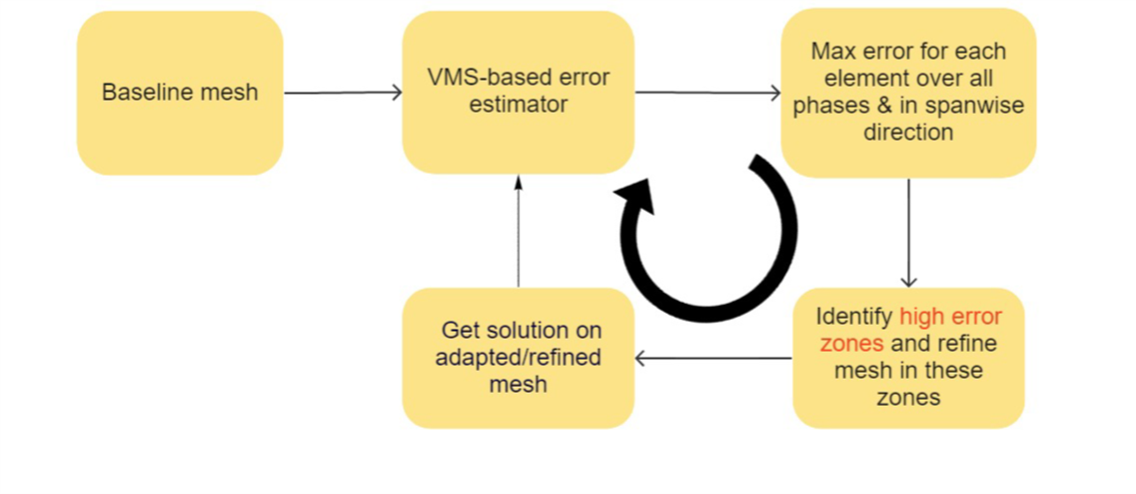
\includegraphics[width=1\textwidth]{figures/adapt_strat/zonal_based.png}
	\caption{Flowchart for zonal adaptation strategy}
	\label{fig:zonal_based_strat}
\end{figure}

For example, a sample of estimated error field in the case of flow over a surging airfoil is shown in Figure \ref{fig:zonal_based_strat_schematic}.
Note that maximum element-level error is obtained for all phases of the cycle and in spanwise direction.
Estimated error is higher in the wake region, as well as in the regions through which the leading edge vortex (LEV) traverses.
High error zones are identified in, and mesh in these zones is refined by a specified factor.

\begin{figure}[H]
	\centering
	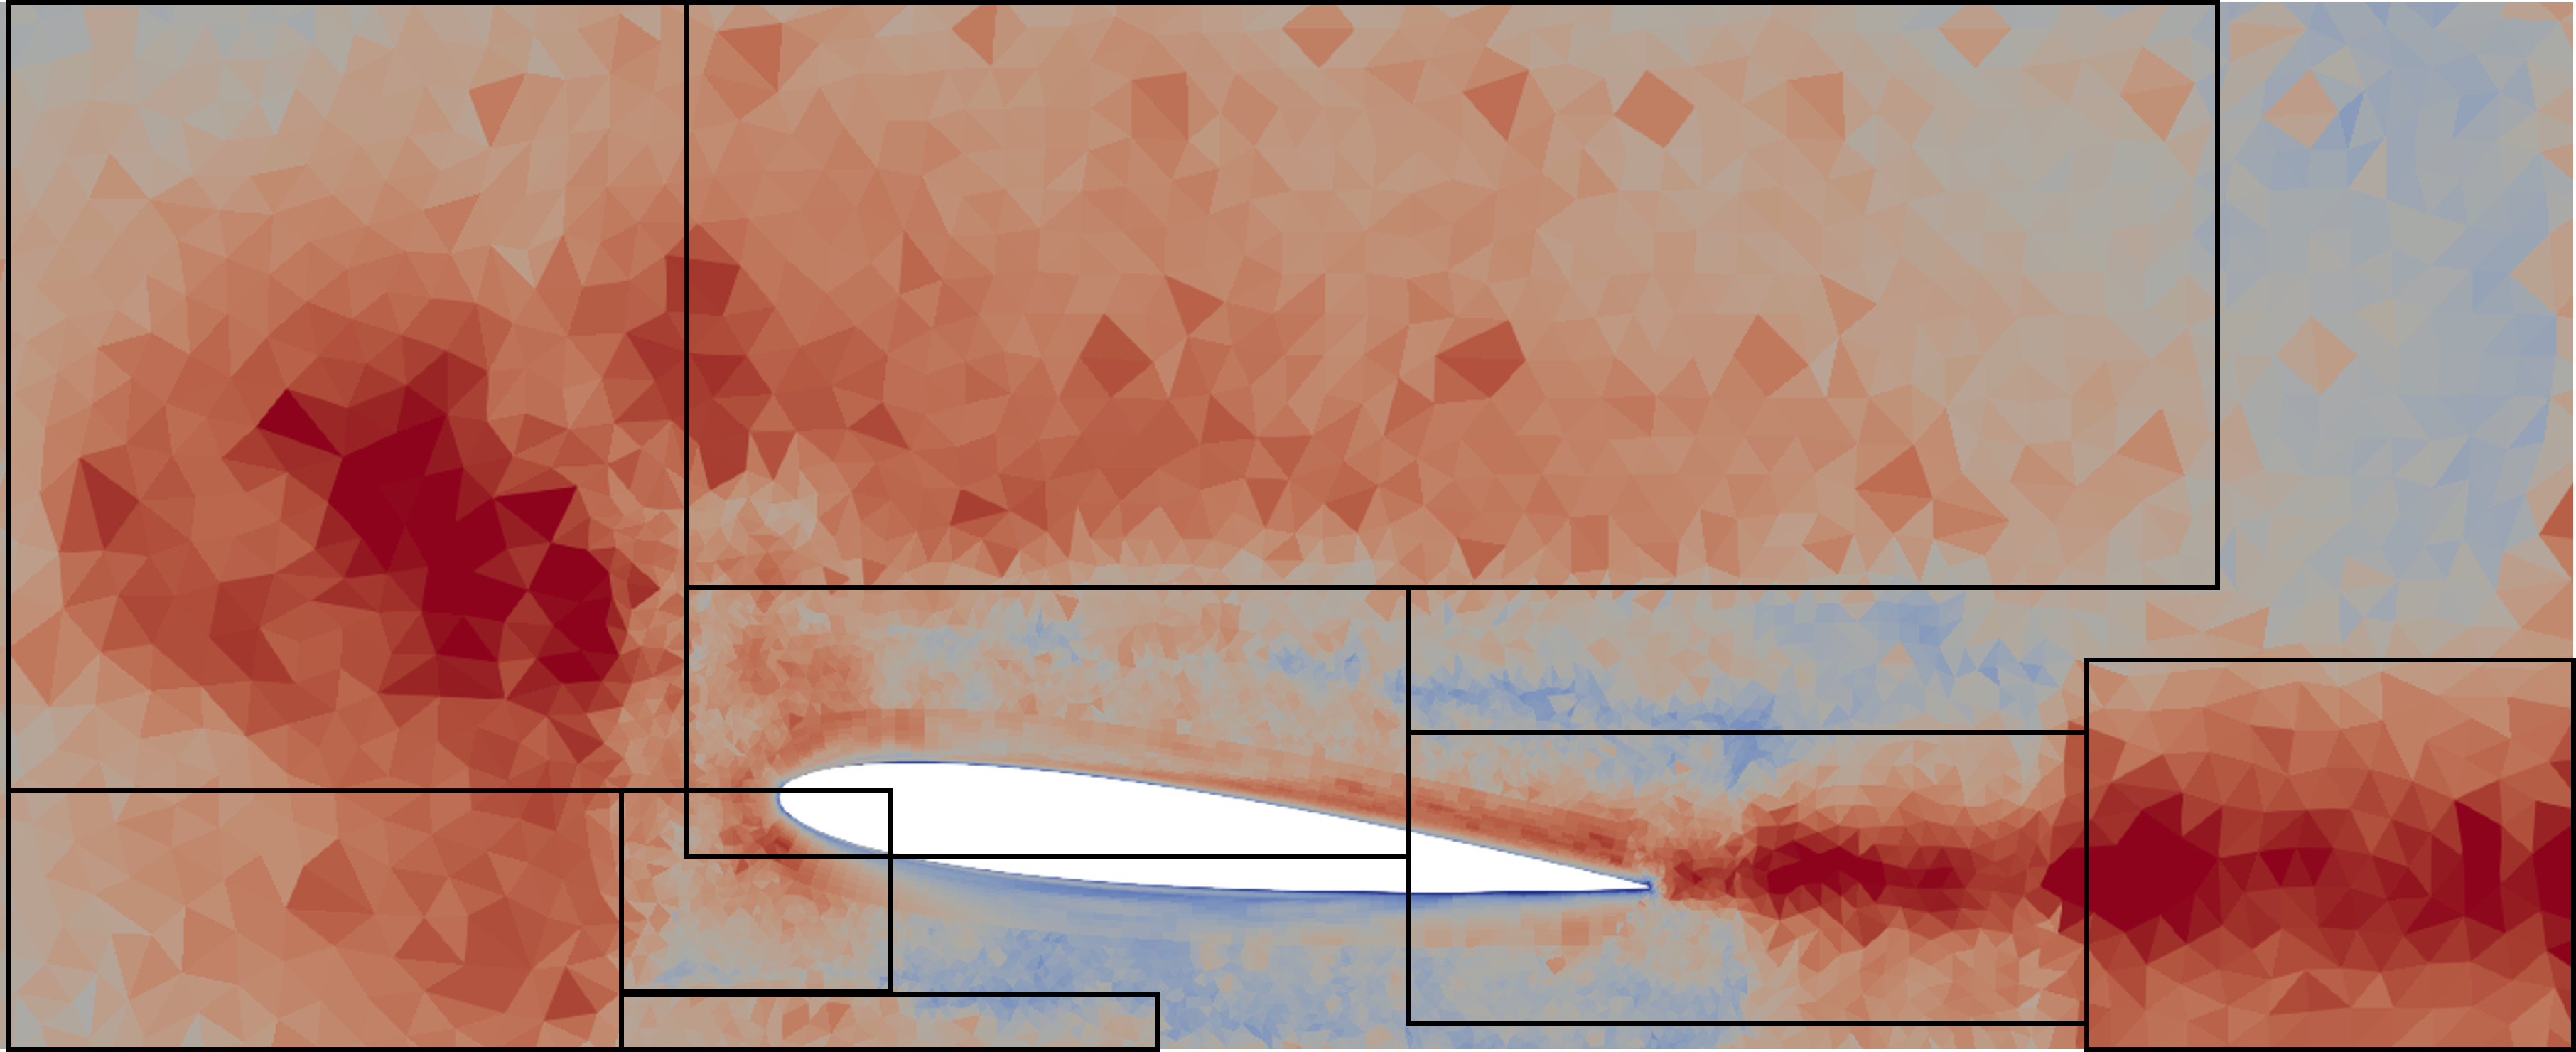
\includegraphics[width=0.75\textwidth]{figures/adapt_strat/zonal_based_schematic.png}
	\caption{Schematic of zonal refinement strategy}
	\label{fig:zonal_based_strat_schematic}
\end{figure}

\subsection{Nodal Size Field-based Adaptation}

The second strategy employs a fully automated mesh adaptation based on the VMS-based error estimator. In this strategy, the estimated error and a specified target error are used to compute the desired mesh size or resolution in a local fashion, i.e., at every mesh vertex. We refer to this as the nodal size field, and the mesh is refined or coarsened based on this nodal size field. 

In this adaptive strategy, the VMS-based error is calculated on the initial mesh. Based on the estimated error, a nodal size field is calculated using the following equation \cite{zhang19}

\begin{equation}
	\frac{e_k}{\tilde{e}_k} = \left(\frac{h_{old}}{h_{new}}\right)^{m+N/2} 
	\label{eq:diez}
\end{equation}

Here, $e_k$ is the measured local error (in the $\HOne$-seminorm) at an element $k$, $\tilde{e}_k$ is the local target error as specified by the user, $m$ is the polynomial order of the approximation space (i.e., $m=1$ for the linear finite elements used currently) , and $N$ is the number of spatial dimensions. $h_{old}$ is the current size of the element, and $h_{new}$ is the desired new mesh size.
This new mesh size at the element level is assembled at the node/vertex level to perform mesh adaptation.
The flowchart for this strategy is shown in Figure \ref{fig:size_based_strat}.

\begin{figure}[H]
	\centering
	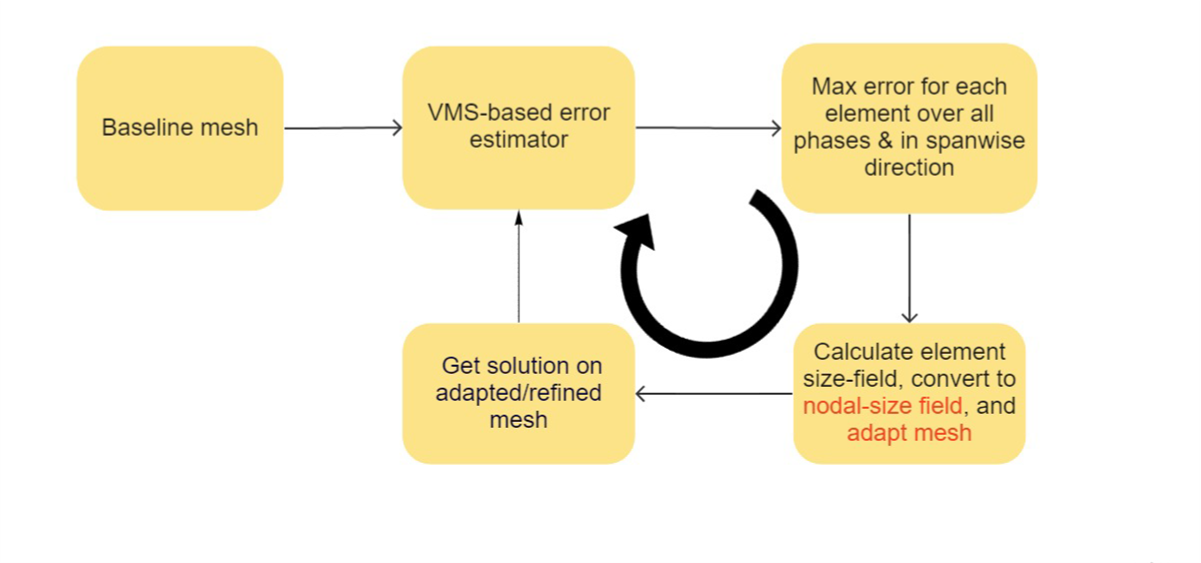
\includegraphics[width=1\textwidth]{figures/adapt_strat/size_based.png}
	\caption{Flowchart for nodal size field-based adaptation strategy}
	\label{fig:size_based_strat}
\end{figure}

\subsection{Feature-based Refinement/Adaptation}

The third strategy is to employ feature-based refinement/adaptation. 
This strategy allows for refinement around the dominant flow features and also along the path/trajectory of such features.
One of the primary flow features is the leading edge vortex (LEV) in the current problems of interest focused on surging airfoils. 
Figure \ref{fig:feature_based_strat_schematic} shows an example of the LEV path and size with respect to the airfoil. 
Mesh refinement is applied along this path as shown by the shaded region.


Two aspects are involved in this strategy: feature detection and tracking, and refinement/adaptation along the feature. These are discussed below.


	
\begin{figure}[H]
	\centering
	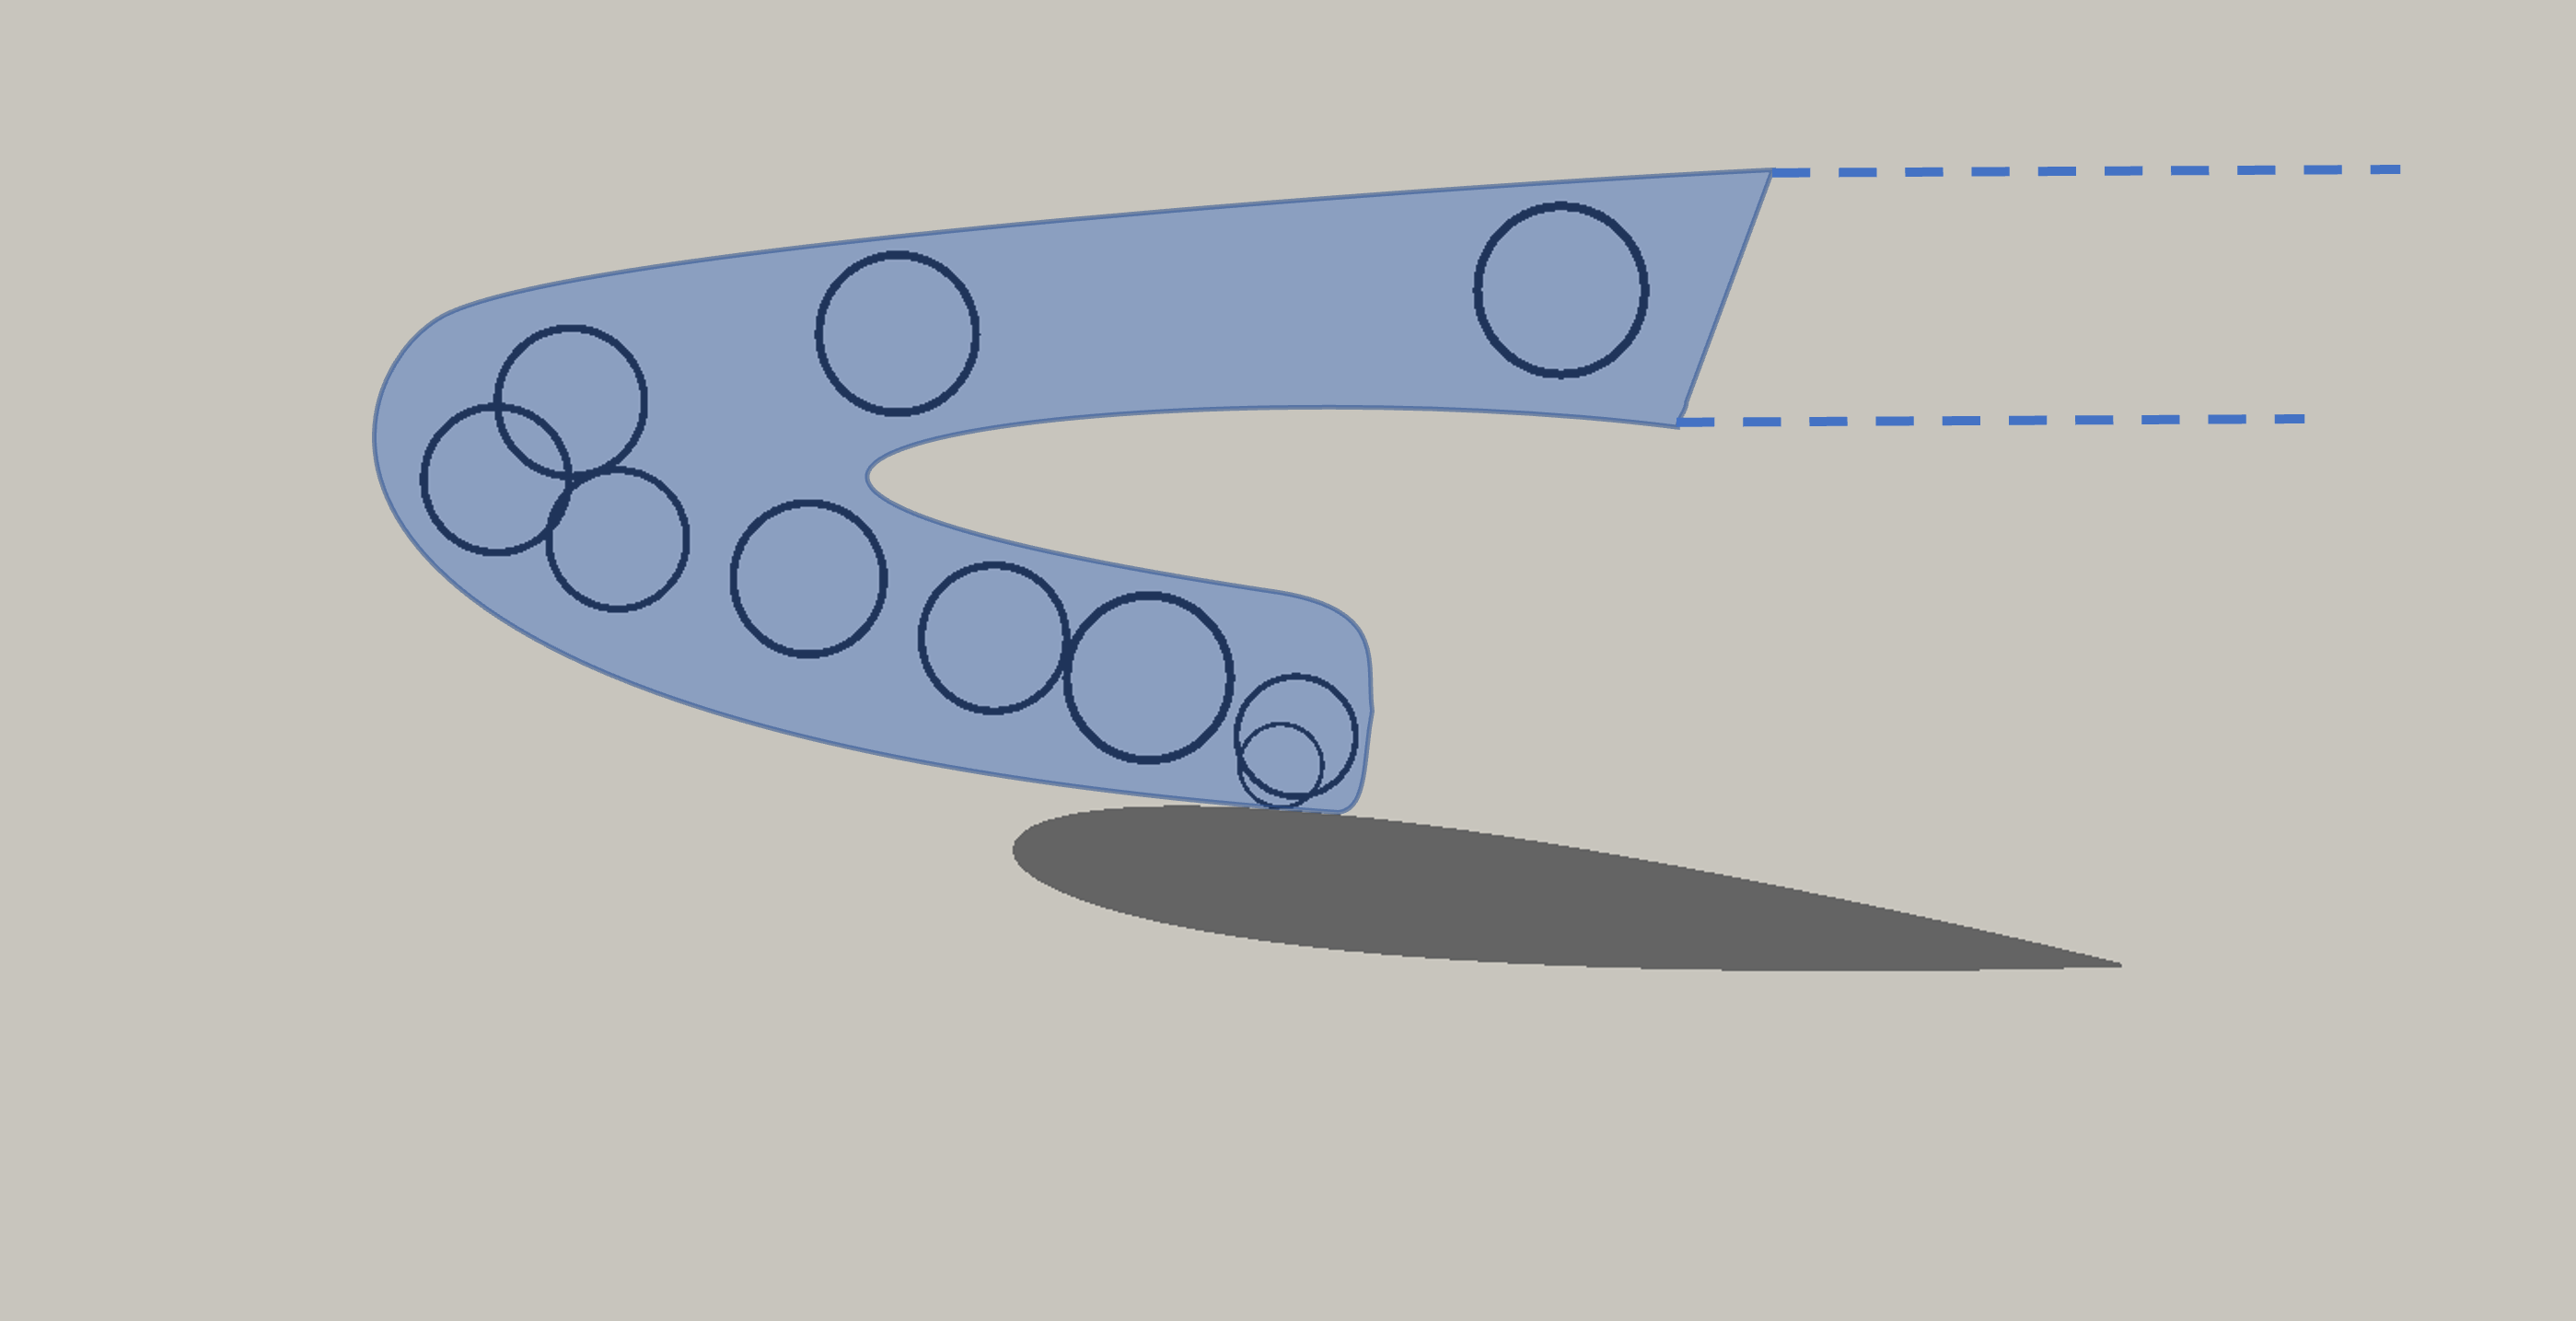
\includegraphics[width=0.75\textwidth]{figures/adapt_strat/feature_based_schematic.png}
	\caption{Schematic of feature-based refinement strategy}
	\label{fig:feature_based_strat_schematic}
\end{figure}

\subsubsection{LEV Detection and Tracking}

%TODO: Show pics and schematics from AIAA paper and presentations (LEV trace)

In this section, we quantify the evolution of the LEV based on its size and position.
In order to do so, phase- and spanwise-averaged data is obtained over multiple cycles.
Note that the LEV forms during the retreating portion of the surging cycle when the boundary layer separates and the separated shear layer rolls up into a vortex. Subsequently, this vortex separates/ejects from the airfoil, and advects with the background flow.
%For example, in Figure \ref{fig:LEV_tracking}, difference between the instantaneous and phase and span averaged vorticity is shown.
Thus, the phase of formation of the LEV is first detected and in subsequent phases the LEV is tracked.
Pressure and velocity data is analyzed to automatically detect the formation of the LEV.
In the retreating portion of the cycle, location with minimum pressure is determined starting at $\psi=180^\circ$.
The first phase at which the minimum pressure location is off the airfoil surface (i.e., away from the airfoil and into the flow) is tagged to be a potential phase for LEV formation.
At this potential phase, velocity profile is obtained over multiple lines passing through the minimum pressure location.
These are radial lines that are taken at an equispaced interval along the azimuth in the plane of the airfoil (note that the data is averaged in the spanwise direction).
These radial lines are shown in Figure \ref{fig:LEV_tracking2}.
Along these lines, at first a relative velocity is computed with respect to the velocity at the minimum pressure location.
Subsequently, normal component of the relative velocity is obtained (i.e., normal to each line), which is the azimuthal or tangential component in the polar coordinate system centered around the minimum pressure location.
The azimuthal component (of the relative velocity) is analyzed against the velocity profile of a Lamb-Oseen vortex.
It is noteworthy that the azimuthal component of the relative velocity along several radial lines at multiple phases in the surging cycle were visually analyzed for different cases and found to fit the Lamb-Oseen vortex model fairly well.

The trace of the LEV is then obtained by applying this process over multiple phases in the surging cycle, which can be used to quantify LEV evolution and to apply feature-based adaptation (as shown above in Figure \ref{fig:feature_based_strat_schematic}).

\begin{figure}[H]
	\begin{subfigure}{0.5\textwidth}
		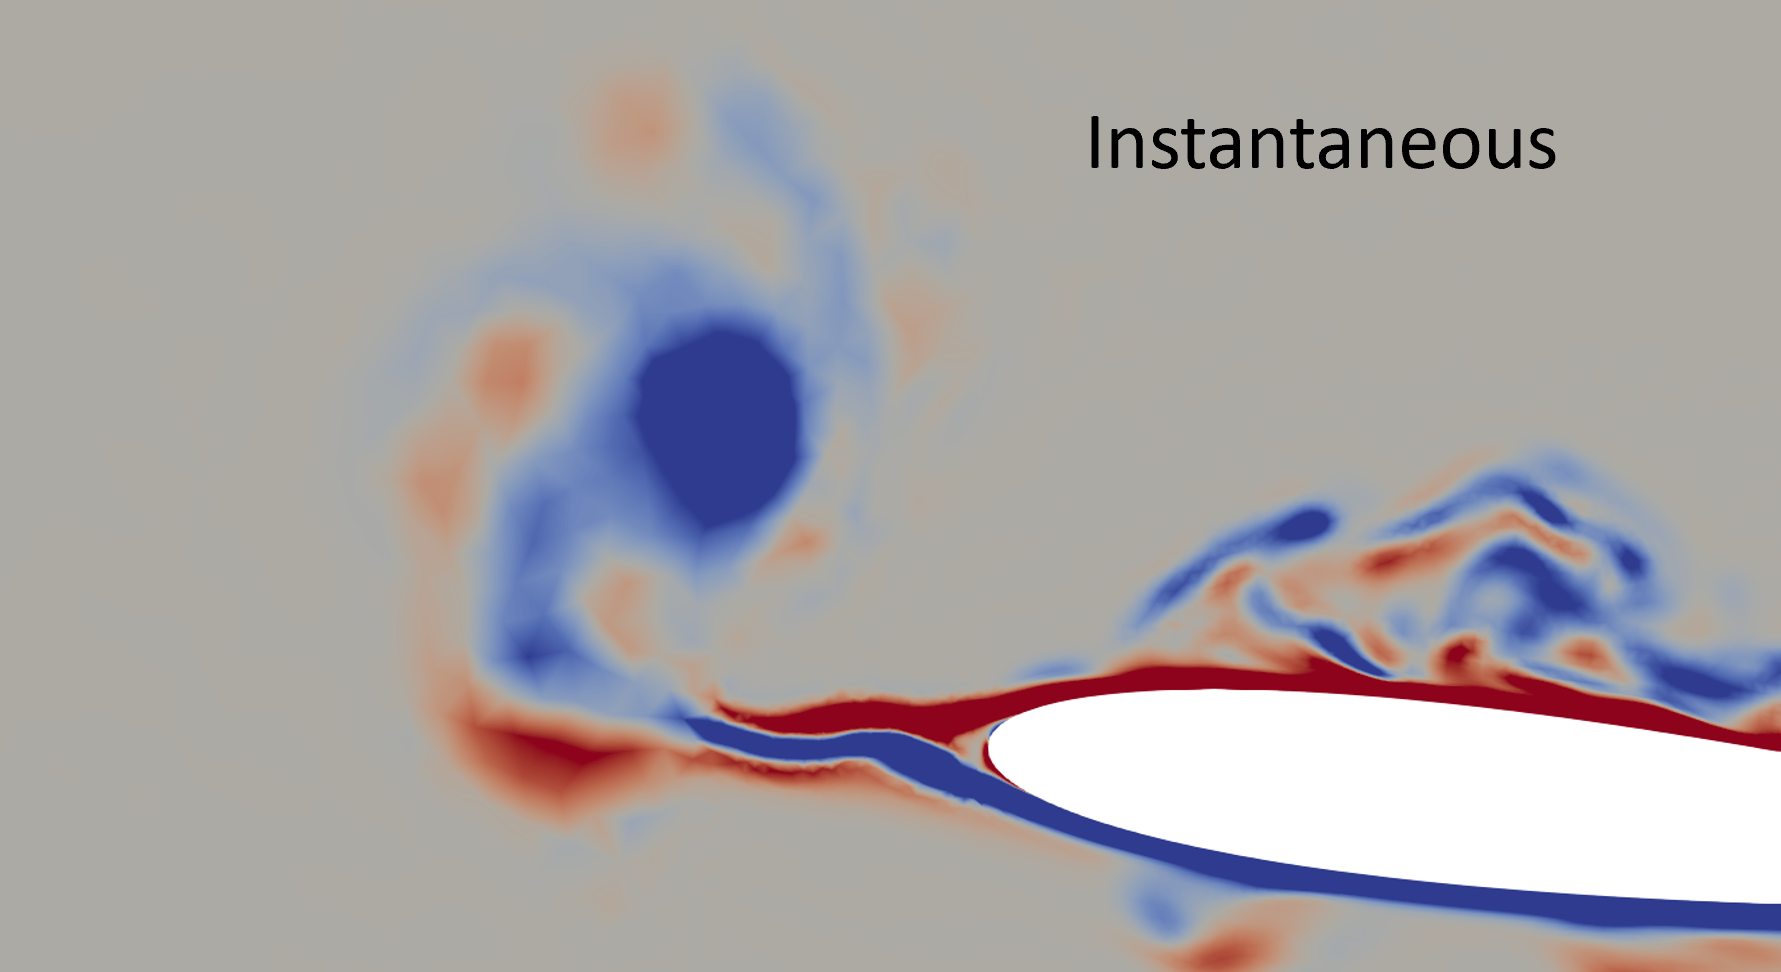
\includegraphics[width=1\textwidth]{figures/adapt_strat/LEV_tracking1.png}
		\caption{Instantaneous LEV}
		\label{fig:LEV_tracking1}
	\end{subfigure}
	\begin{subfigure}{0.51\textwidth}
	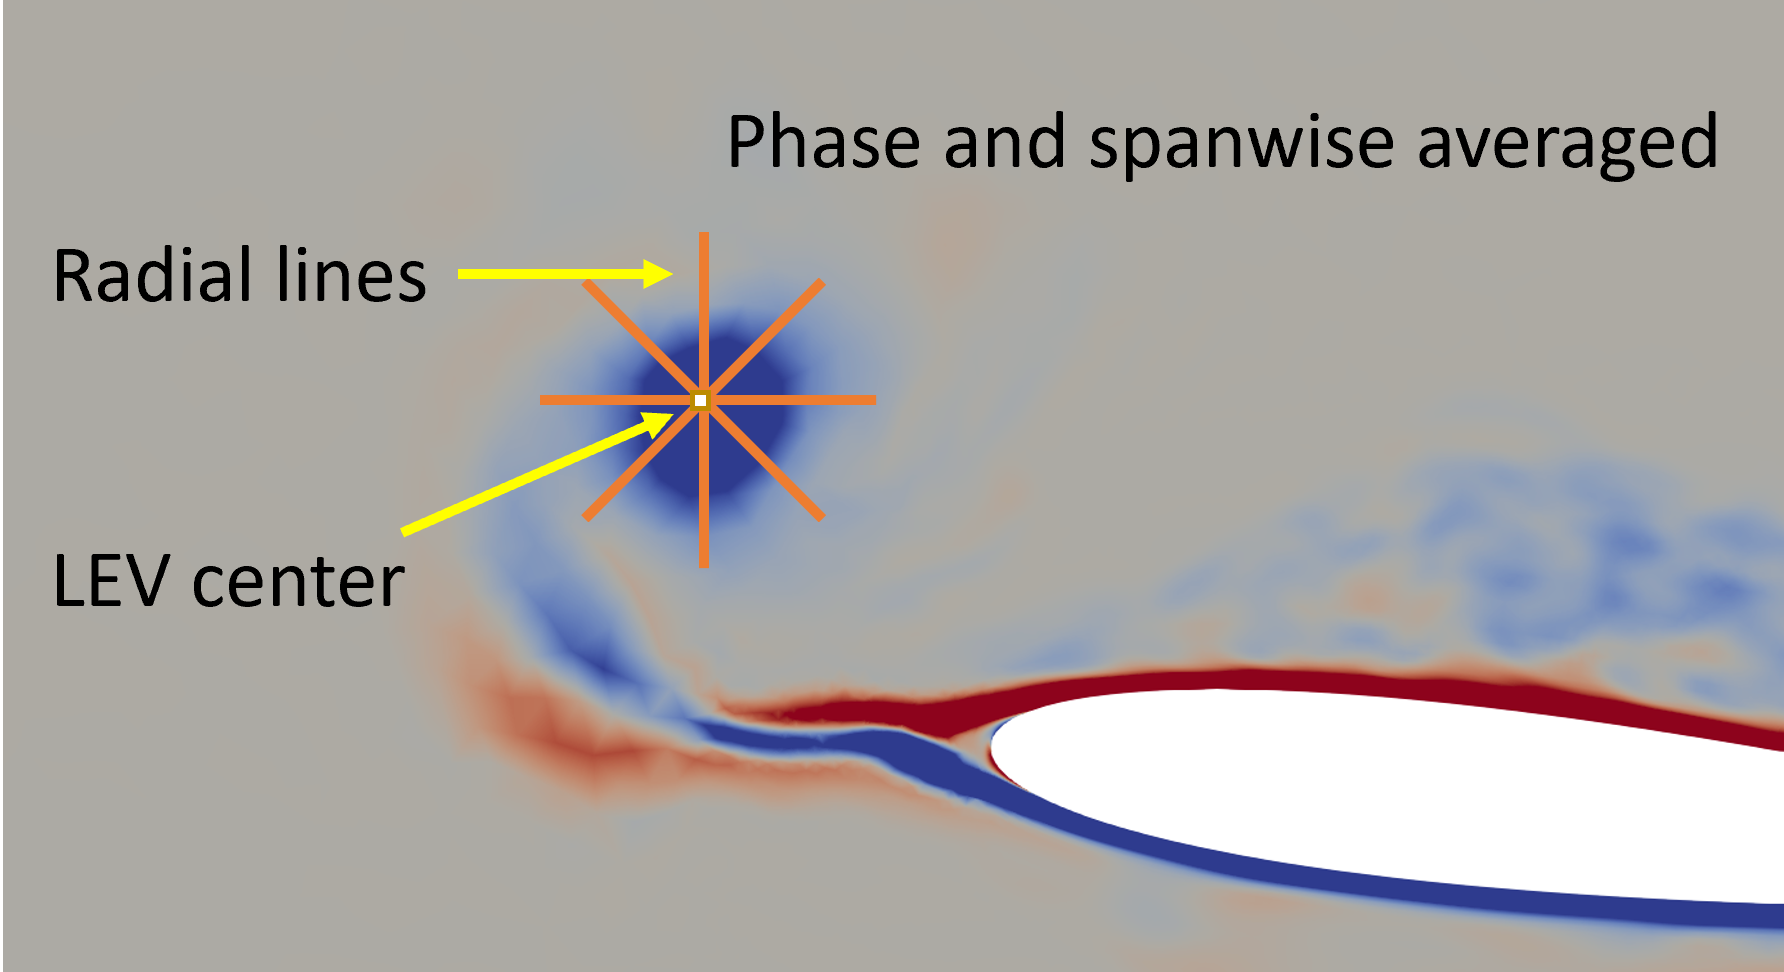
\includegraphics[width=1\textwidth]{figures/adapt_strat/LEV_tracking2.png}
	\caption{Averaged LEV}
	\label{fig:LEV_tracking2}
	\end{subfigure}

	\centering
	\begin{subfigure}{0.5\textwidth}
	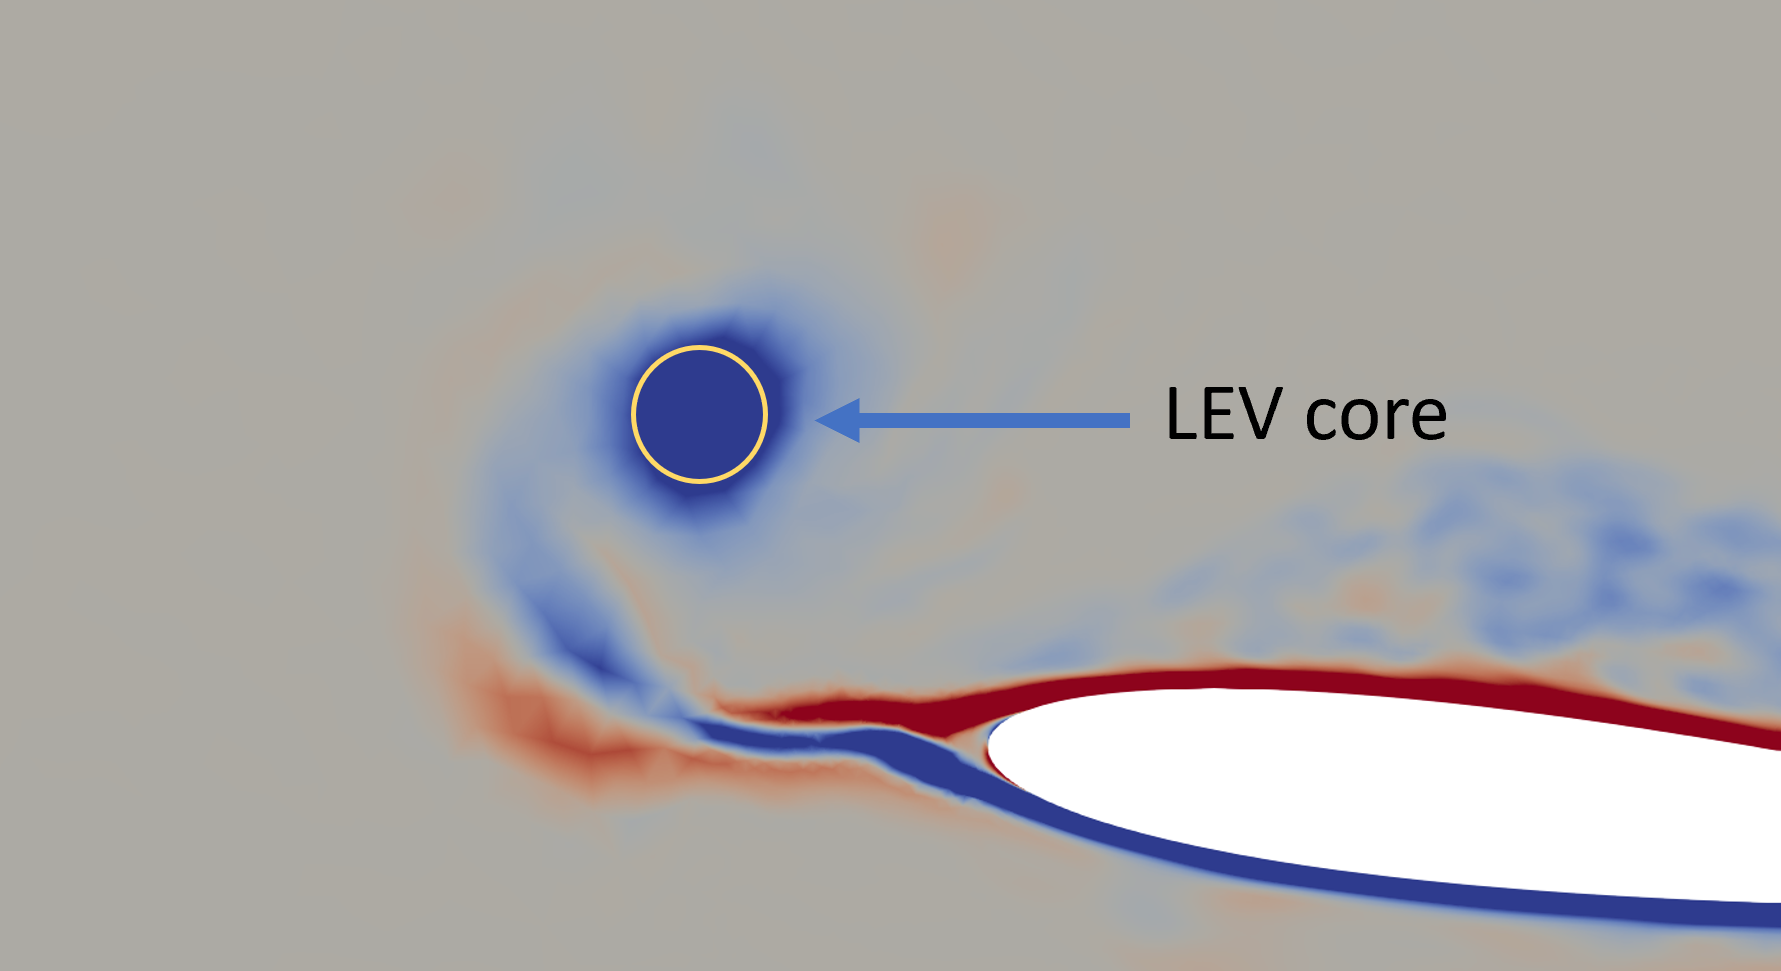
\includegraphics[width=1\textwidth]{figures/adapt_strat/LEV_tracking3.png}
	\label{fig:LEV_tracking3}
    \caption{Averaged LEV with core radius}
\end{subfigure}
	
	\caption{Schematic of LEV quantification}
	\label{fig:LEV_tracking}
\end{figure}


\subsubsection{LEV-based Refinement/Adaptation}

For a given simulation, we can follow three steps: (i) get information on the approximate path and extent that a certain feature will follow, (ii) estimate the error along this path/region, and (iii) perform refinement/adaptation along this path.
For example, in the case of flow over surging airfoils, the path and size of LEV over a surging cycle is used to detect portions in the mesh where refinement is applied.
Similarly, other features such as trailing edge vortex (TEV) can also be targeted using such a feature-based refinement. The flowchart for this strategy is shown in Figure \ref{fig:feature_based_strat}.

\begin{figure}[H]
	\centering
	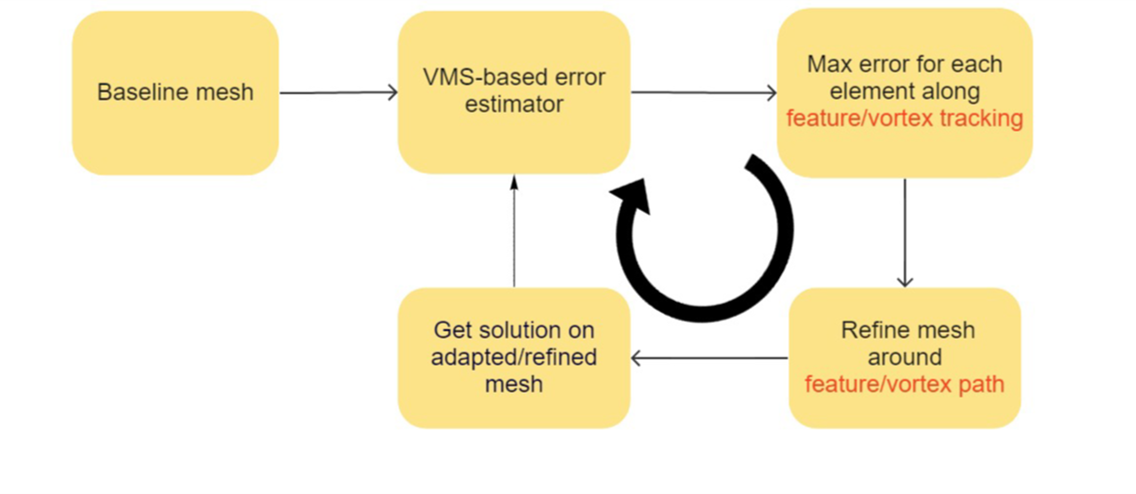
\includegraphics[width=1\textwidth]{figures/adapt_strat/feature_based.png}
	\caption{Flowchart for feature-based refinement strategy}
	\label{fig:feature_based_strat}
\end{figure}


